\section{The choice of development process}
The choice of a development process is crucial for every project~\cite{book:software-engineering} 
and many factors such as project size and scope, team members skills and time resources have to 
be taken into consideration in order to make a good choice. The choice of the development process 
will affect planning and many other aspects of the teamwork. The following section describes
which development processes we have considered using and the reasons behind our final choice.

\subsection{Waterfall}
The Waterfall model (figure \ref{fig:designmodel-waterfall}) is a strict top-down design process. It features detailed planning, design and
documentation before design. This model is useful when going back and changing requirements is
costly or impossible. This does however require that all needed features and requirements are known
early on. The model was originally used for hardware design and when the first software projects 
appeared it was simply adapted. Many argue that the Waterfall model is bad for software design, seeing
as the developers cannot predict all problems or additional requirements before reviewing a working
prototype of the final product. Customers also often have changing requirements under development.
The Waterfall model works best for expensive projects where problem prediction and initial correct design
is vital before implementation is started.
\begin{figure}[h!]
\centering 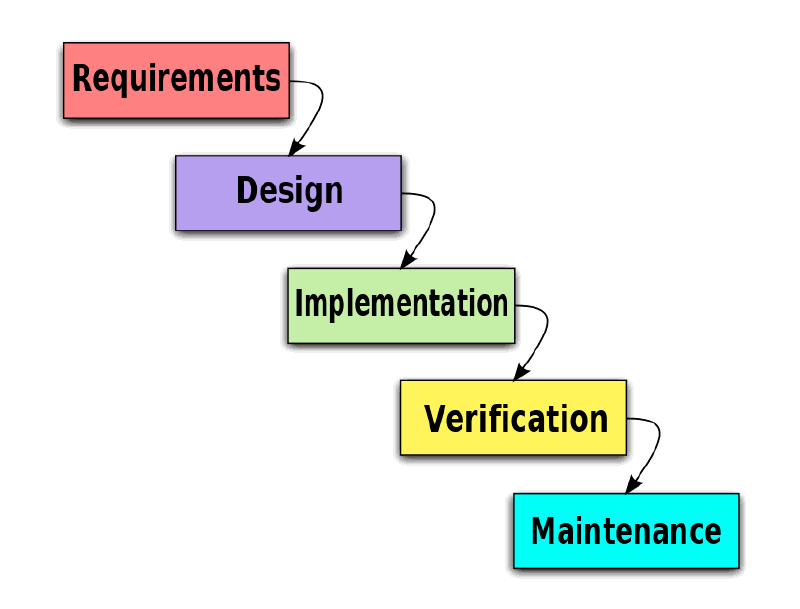
\includegraphics[scale=0.30]{img/designmodel-waterwall} \caption{The Waterfall model~\cite{link:wiki}}
\label{fig:designmodel-waterfall}
\end{figure}

\subsection{Scrum} 
\label{section:scrum}
Scrum is an Agile software development process. The Scrum approach uses repetitive iterations (called
Sprints in the Scrum etymology) to design, implement and refine a product. Figure \ref{fig:designmodel-scrum} shows
how the Scrum iterative process works. Each iteration improves, fixes and adds new features to the previous iteration.
A key feature of Scrum is that the customer can change their mind on what they want or need. Scrum focuses on frequent 
group meetings and splitting big tasks into smaller, manageble tasks for small groups of programmers. Because of the
frequent meetings it promotes verbal communication in the group.
\begin{figure}[h!]
\centering 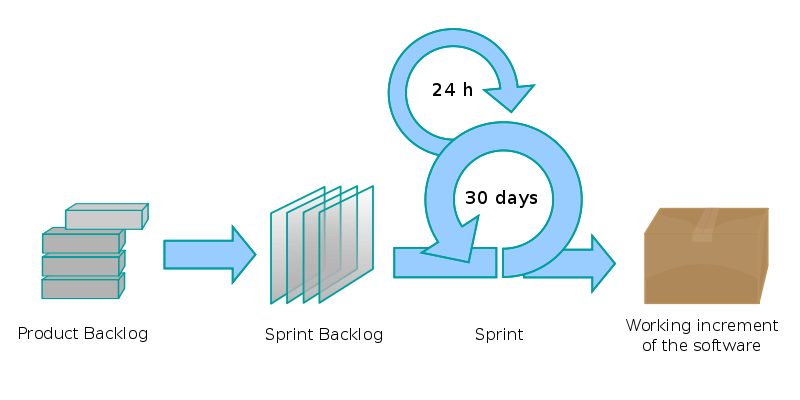
\includegraphics[scale=0.4]{img/designmodel-scrum} \caption{The Scrum process~\cite{link:wiki}}
\label{fig:designmodel-scrum}
\end{figure}

\subsection{Extreme Programming (XP)}
Extreme Programming (figure \ref{fig:designmodel-xp}) is a development methodology that is designed for best software quality and
quick responsivness to changing customer requirements. It is also an Agile Development method like
Scrum and therefore shares certain similarities to that development method. It promotes rapid
development and allows the customer to change his/her mind or request new features throughout
the development of the software. Typical elements for XP are pair programming, unit testing,
lazy programming, simplicity and expecting changes in customer requirements as time passes
and the problem is better understood. Several pitfalls include buggy and unstable code or lack of
overall design specification. Extreme programming is best suited for small projects for prototyping
where the customer is not entierly sure what he or she wants.
\begin{figure}[h!]
\centering 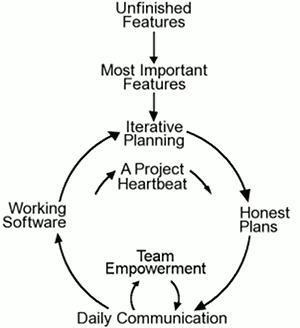
\includegraphics[scale=0.75]{img/designmodel-xp} \caption{Extreme Programming~\cite{link:xp}}
\label{fig:designmodel-xp}
\end{figure}

\subsection{Agile Unified Process}
The AUP (short for Agile Unified Process) shown in figure \ref{fig:designmodel-aup} offers a simple and easy to understand approach for software
development. It is a simplified version of the Rational Unified Process. Key features are simplicity, 
customization and focus on the task on hand instead of everything that may happen. It features
several internal development iterations before producing a customer release. AUP focuses on quality
insurance and works best for projects that is going to be used by a large public and a working, bugfree
product is important.
\begin{figure}[h!]
\centering 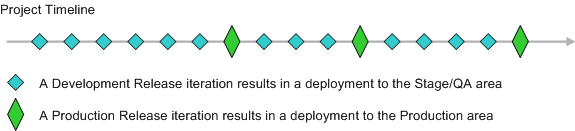
\includegraphics[scale=0.65]{img/designmodel-aup} \caption{AUP development iterations\cite{link:wiki}}
\label{fig:designmodel-aup}
\end{figure}

\subsection{Spiral Model}
The Spiral development methodology (figure \ref{fig:designmodel-spiral}) combines the advantages of both the top-down approach 
from Waterfall and the bottom-up concept of prototyping. It does this by using an iterative development
approach and by controlling it through the systematic Waterfall model. A strong advantage of the Spiral lifecycle is that it
allows new features and requests to be integrated as soon as they come avalible or known. Other key 
features of the model is risk analysis, strict system design specifications and prototyping. The Spiral model
 is best suited for large, expensive and complicated projects.
\begin{figure}[h!]
\centering 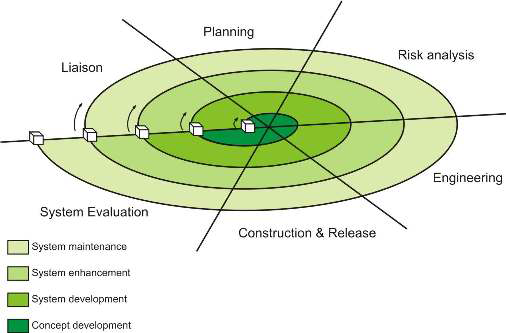
\includegraphics[scale=0.85]{img/designmodel-spiral} \caption{The Spiral model~\cite{link:spiral}}
\label{fig:designmodel-spiral}
\end{figure}

\subsection{Conclusions}
At week 1 we initially chose Scrum as our development process. The reasons behind this choice were the iterative nature
of our work schedule and of our weekly meetings with the customer during which we had to present a new version
of the prototype each time. Moreover everyone in the team had some experience with Scrum from previous projects.

After a few weeks of development however, we began to wonder if the Scrum model did not fit perfectly to our project.
This was due to the fact that especially on the 'social' part this project was much like a software research project
so the specifications and the requirements for the product were not clearly set early on, but instead unfolded little
by little during our meetings with the customer thanks to his feedback on our prototypes and documentation.
This led to some of the code and documentation that we produced to be scrapped during later iterations,
but also and especially to some delays in the overall system design. These scrapped designs are included in Appendix B.

We researched then some other development processes, namely Extreme Programming and Spiral. The Spiral model 
did not suit our project, it is rather meant for larger projects with many employees. XP didn't fit us either as we needed 
a process that produced more documentation. In the end we continued to use Scrum after making some changes to the 
process itself.

%Roles of each member? Scrum Master, Team Leader, Customer Relations, etc.
\section{Project Roles}
\begin{itemize}
	\item \textbf{Scrum Master:} \henrik\newline
	Took care of managing the Scrum process.
	
	\item \textbf{Customer Relations:} \henrik\newline
	Took care of contacting the customer and arrange meetings.

	\item \textbf{Arduino developers:}\anders, \bjornar ~and \johan\newline
	Took care of developing the Arduino code and the Java library that takes
	care of estabilishing connections with Arduino.

	\item \textbf{Android developers:}  \emanuele~and \henrik\newline
	Took care of the designing the user interfaces for the Android applications
	as well as designing the Java library that allows Android applications
	to exchange social data.
	
	\item \textbf{Quality Assurance:} \johan, \asbjorn~and \jonas\newline
	Ensure that every package and module in the system passes the requirement tests
	that were setup in the Requirements section. The final product must statisfy certain
	requirements before we can deliver it to the customer.

	\item \textbf{Documentation:} Everyone\newline
	Every team member produced documentation regarding their work areas and
	collaborated in writing the reports.

	\item \textbf{Supervisor:} Njaal C. A. Gjerde\newline
	Documentation support and report revisions. Every two weeks we would meet the project supervisor
 	and he would give us feedback and suggestions for improvements for the project process and documentation.

	\item \textbf{Customer:} Babak A. Farshchian at SINTEF \newline
	Every week friday at 14:15 we would meet with the customer. After a progress update we would show the results
	of the work we had done earlier that week. The customer would then give us guidelines and requests for what
	he would like to have finished for the next sprint. The duration of the meetings with the customer varied anything
	from 15 minutes to two hours, depending on the amount of topics that need to be discussed.
\end{itemize}

\section{Project management tools}

To help us in using Scrum we chose an online tool called ScrumDo (figure \ref{fig:mgmt-scrumdo}).
This tool has features for most if not all parts of the Scrum process. Using this tool
consistently will be our main method of maintaining and separating packages from
the WBS (Work Breakdown Structure). In the context of ScrumDo and
Scrum these low level work packages are called stories and are moved
accordingly from "ToDo" over to "In progress"
and eventually to "Done" areas.
	
\begin{figure}[h!]
\centering 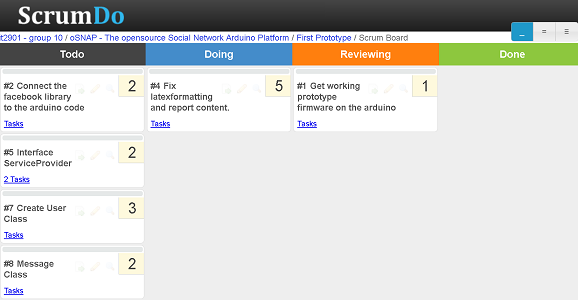
\includegraphics{img/mgmt-scrumdo} \caption{A screen capture of the Scrum Board in ScrumDo \cite{link:scrumdo}}
\label{fig:mgmt-scrumdo}
\end{figure}

\subsection{Software and hardware development tools}
Various software tools were used for this project.

These include:\newline
\begin{itemize}
	\item \textbf{IDE for Coding:} \newline
	NetBeans and Eclipse for Java development. SublimeText amd Arduino for embedded C development.

	\item \textbf{Collabaration tools:} \newline
	For our code repository we decided to use GIT\cite{link:git}. GIT is a fast, scalable, distributed revision control system 
	with an unusually rich command set that provides both high-level operations and full access to internals. Also 
	several team members had experience with GIT through other projects which was a significant factor for 
	this choice.

	We used Skype for instant message communication.

	\item \textbf{Libraries and external software:} \newline
	 Facebook Android SDK, Android SDK, RXTX

	\item \textbf{\LaTeX{} and Google Documents:} \newline
	Used for producing documentation. Google Documents for realtime documentation collaboration.

	\item \textbf{Google Drawing:} \newline
	Google Drawing was used to generate the various figures and graphics used throughout the documentation.

	\item \textbf{Microsoft Visio:} \newline
	Used to create various charts and diagrams throughout the documentation. 

\end{itemize}

The project required use of various hardware devices like Arduino boards and Android mobile phones. SINTEF kindly arranged for us so that we could borrow and order Arduino equipment through them for making the prototypes. The team used Android emulators and their own phones for running, testing and prototyping the system.

\section{Risk analysis and mitigation strategies}

This text will highlight different realistic risks that may occur during development
that can to some degree jeopardise the process or the final product.
A table with weighted risks and relative mitigation and remedial actions follows.

\begin{itemize}

\item \textbf{Dropouts}\newline
The risk of people dropping the course or otherwise not being able to complete it as part
of the group. This can be caused by sickness as well.

\item \textbf{Arduino hardware}\newline
Our handed out Arduino equipment can fail, due to malfunctioning or wrong usage.
There is also the possibility that some of the hardware can be lost while we work with it at home.

\item \textbf{Deadlines}\newline
Throughout the course there is multiple deadlines that must be met. Failure to meet
these limits will have huge impacts on the grading and could possibly fail the group.

\item \textbf{Choosing wrong frameworks}\newline
We will necessarily have to build parts of our software around existing open source
frameworks to limit effort required by the task. If at a later point we have severe limitations
on our possibilities due to these frameworks the product could result poorer in features than
we originally planned. The impact can be negligible if other solutions are found.

\item \textbf{Design problems}\newline
It could happen that the system design is late on schedule and delays other parts of the project
including testing and documentation. Also during development features have to be constrained due to problems
or resource limitations. This could cause the final product to not satisfy the customer.
If we can find work-arounds and compromises, then the problem will not have a big impact on the process.

\item \textbf{Wireless connectivity}\newline
If the Arduino chip modules (called shields) for Bluetooth and other network interfaces were too
hard to implement we would have to reconsider wireless connectivity as an option.
We set the 'get wireless to work' deadline to be one month. If we can't get it working
by that time we will have to use cabled connections instead and that would result clumsy
for a lot of concepts.
\end{itemize}

\begin{table}
	\begin{center}
		\caption{Risk Analysis}
		\rowcolors{1}{white}{lightgray}
		\begin{tabular}{| p{2.1cm} | l | l | l | p{2.8cm} | p{3cm} |}
		\hline

\textbf{Description} & \textbf{Likelihood} & \textbf{Impact} & \textbf{Risk} & \textbf{Mitigation} & \textbf{Remedial Action}\\ \hline

Evolving requirements	& 8 & 9 & 9 & Specify a set of requirements that both the customer and the devolopers agree on.
					& Meetings with the customer to agree on revisions in the requirements \\ \hline

Missing Hardware		& 7 & 6 & 7 & Have control over who has what and keep an inventory list.
					& Get new hardware if possible. We also have multiple backup Arduino modules ready. \\ \hline

API Trouble			& 6 & 5 & 6 & Limit the scope to documented open source APIs.
					& Investigate alternative solutions. Limit impact on productivity. \\ \hline

Sickness 			& 5 & 4 & 5 & Keep contagious sicknesses at home.
					& If the sickness is prolonged work tasks must be re-arranged appropriately. \\ \hline

Low product quality		& 3 & 6 & 4 & Thorough test plans  and QA. Avoid late features implementation.
					&  Workaround problems at critical junctions in the process.\\ \hline

Arduino Malfun.		& 2 & 3 & 3 & Treat hardware properly. Do not eat or drink nearby.
					&  Get new hardware if possible. We also have multiple backup Arduino modules ready. \\ \hline

%Wireless Connect.		& Low & High & Med & Get it working & Switch to cable connection \\ \hline

%Mid-Sem Deadline		& Low & High & Med & Produce good documentation and begin early on reports.
%					&  Consult with student assistants.\\ \hline
			
%Final Deadline		& Low & High & Med & Consistent work throughout the semester. Avoid last-minute feature implementation.
%					&  Deliver the product in the best state possible.\\ \hline

		\end{tabular}
	\end{center}	
	\label{table:riskanalysis}
\end{table}

Concluding, most care should be put in the choice of existing frameworks and in early planning
and documentation efforts to avoid later problems related to the implementation and report delivery.


\section{Resources}
A meeting table was arranged during the first meeting. Team members
have weekly meetings on Monday, Wednesday and Friday at twelve o'clock.
Meetings with the client were arranged for each Friday at two fifteen (14:15).
Appendix C summarizes the meeting minutes for these meetings. In addition we
have weekly status reports for project development progress in appendix A.

The team exchanged both e-mails and mobile numbers. A permanent Skype
group chat on which we meet on a daily basis was set up, a mailing
list was also created. Several documents of interest to the group
were made available to everyone using Google Documents.

\subsection{Resource Distrubution}
We estimate 20 hours work per person each week. With a group of 7 members this means we have
140 manhours available each week. Since the project is approximately 17 weeks long, we have

\begin{equation}
17 weeks * 140 hours = 2380 hours
\end{equation}

%\subsection{Work Breakdown Structure}

\begin{figure}[h]
\centering 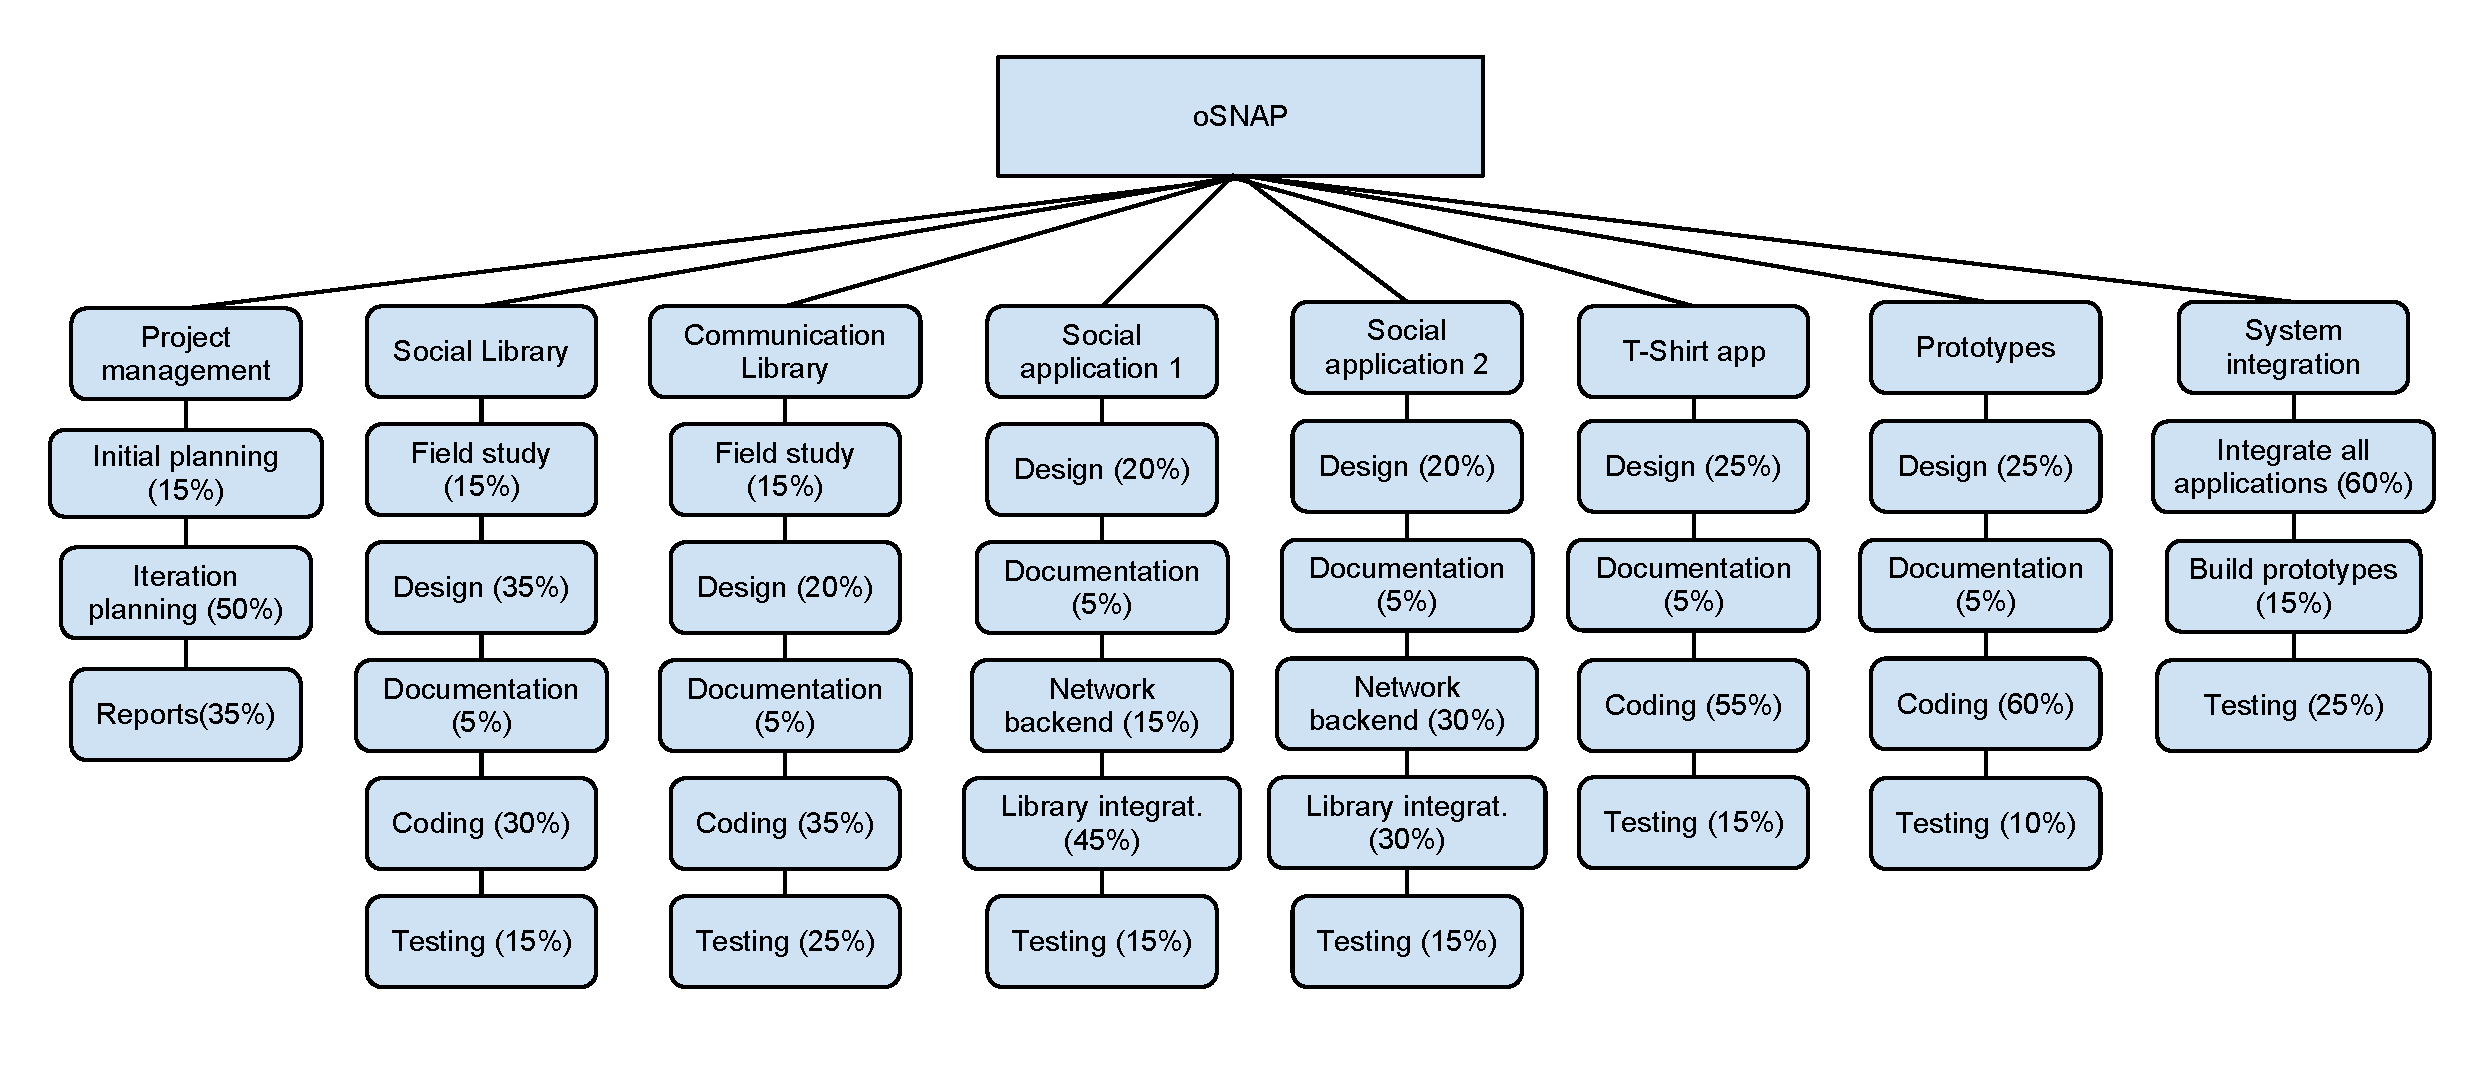
\includegraphics[width=1.1\textwidth]{img/mgmt-wbs.pdf} \caption{Work Breakdown Structure}
\label{fig:mgmt-wbs}
\end{figure}

%\subsection{Milestones}
\begin{table}[h]
	\begin{tabular}{| l | r |}
		\hline

		\textbf{Description} & \textbf{Estimated completion date} \\
		\hline

		Working Social networks communication & 2-2-2012 \\
		\hline

		Preliminary project report & 6-2-2012 \\
		\hline

		Working Android Arduino wireless comm. & 10-2-2012 \\
		\hline

		System design completed & 2-3-2012 \\
		\hline

		Mid. semester project report & 9-3-2012 \\
		\hline

		Communication library completed & 16-3-2012 \\
		\hline

		Social library completed & 30-3-2012 \\
		\hline

		Last supervised project report & 16-4-2012 \\
		\hline

		Prototype completed & 11-5-2012 \\
		\hline

		Project delivery & 25-5-2012 \\
		\hline

	\end{tabular}
	\caption{Project milestones}
	\label{tbl:milestone}
\end{table}

%\subsection{Gantt Diagram}

\begin{figure}[h]
\centering 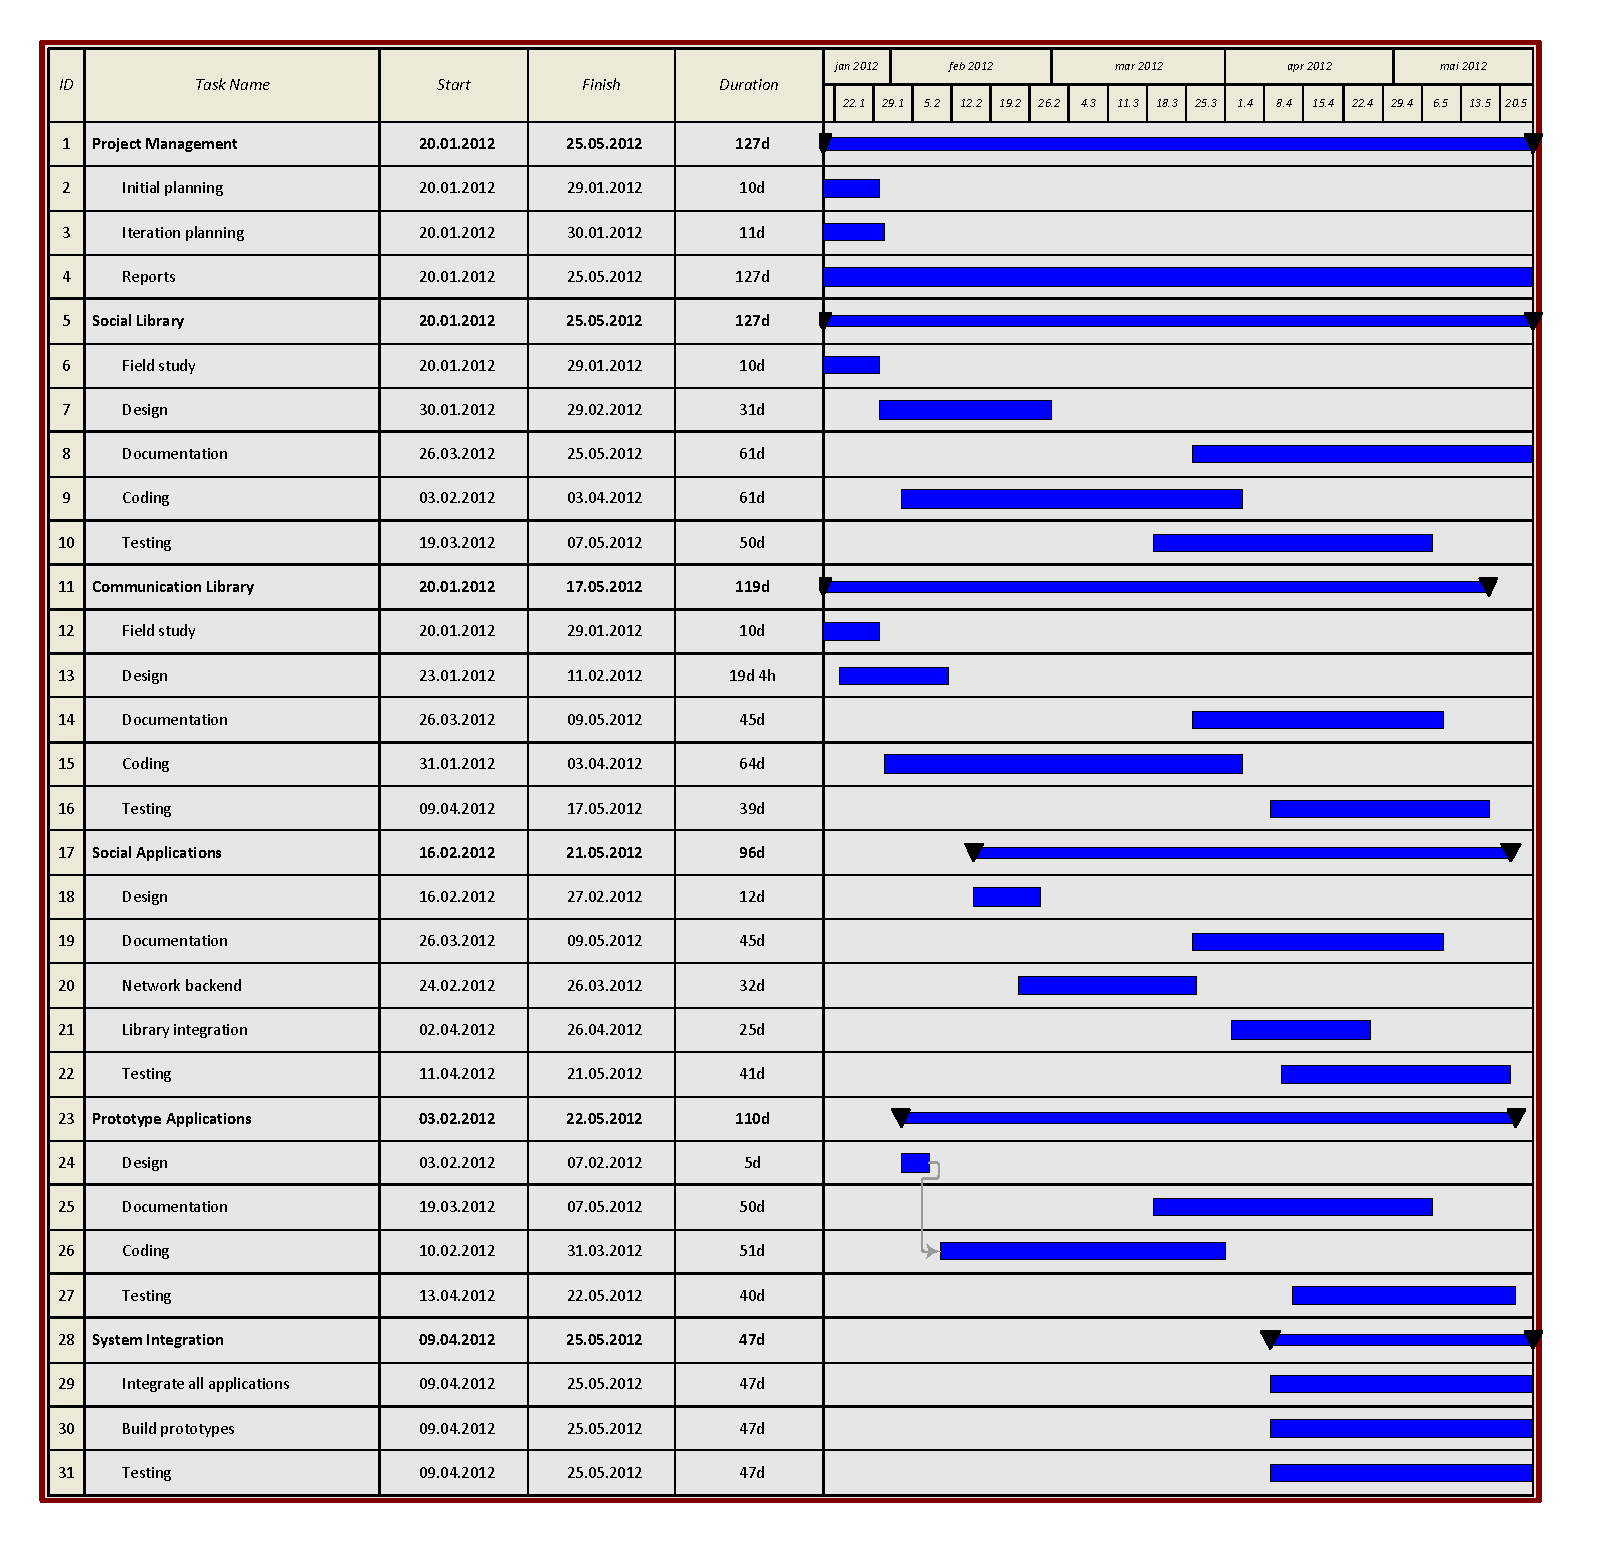
\includegraphics[angle=270, width=1\textwidth, trim=0mm 0mm 47.5cm 0mm, clip]{img/mgmt-gantt.pdf} \caption{Gantt Diagram - part 1}
\label{fig:mgmt-gantt-1}
\end{figure}

\begin{figure}[h]
\centering 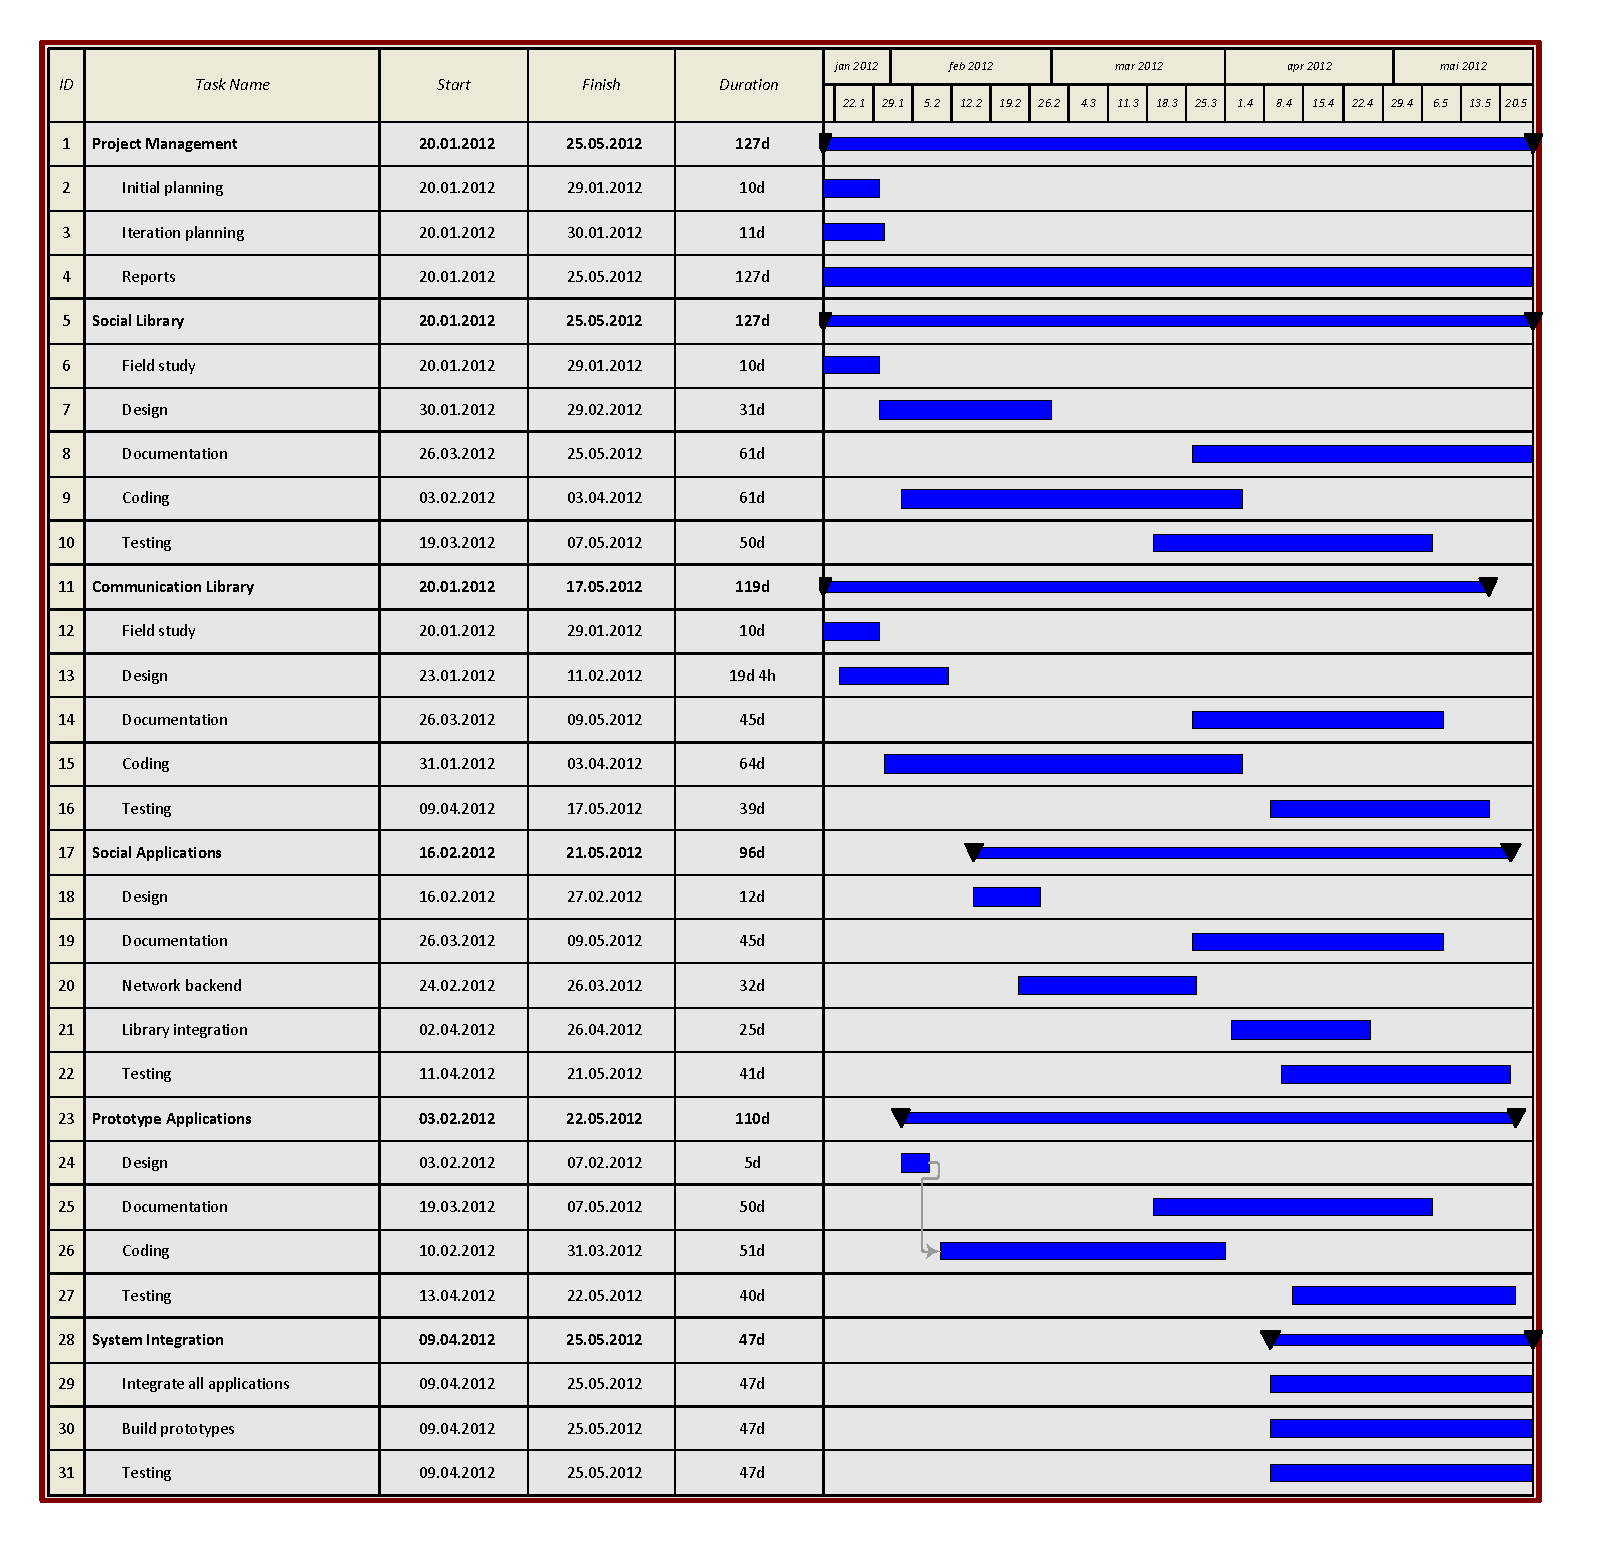
\includegraphics[angle=270, width=1\textwidth, trim=45.5cm 0mm 0mm 0mm, clip]{img/mgmt-gantt.pdf} \caption{Gantt Diagram - part 2}
\label{fig:mgmt-gantt-2}
\end{figure}
